\documentclass{beamer}
\usepackage{amsmath,graphics}
\usepackage{amssymb}

\usetheme{default}
\usepackage{xcolor}

\definecolor{solarizedBase03}{HTML}{002B36}
\definecolor{solarizedBase02}{HTML}{073642}
\definecolor{solarizedBase01}{HTML}{586e75}
\definecolor{solarizedBase00}{HTML}{657b83}
\definecolor{solarizedBase0}{HTML}{839496}
\definecolor{solarizedBase1}{HTML}{93a1a1}
\definecolor{solarizedBase2}{HTML}{EEE8D5}
\definecolor{solarizedBase3}{HTML}{FDF6E3}
\definecolor{solarizedYellow}{HTML}{B58900}
\definecolor{solarizedOrange}{HTML}{CB4B16}
\definecolor{solarizedRed}{HTML}{DC322F}
\definecolor{solarizedMagenta}{HTML}{D33682}
\definecolor{solarizedViolet}{HTML}{6C71C4}
%\definecolor{solarizedBlue}{HTML}{268BD2}
\definecolor{solarizedBlue}{HTML}{134676}
\definecolor{solarizedCyan}{HTML}{2AA198}
\definecolor{solarizedGreen}{HTML}{859900}
\definecolor{myBlue}{HTML}{162DB0}%{261CA4}
\setbeamercolor*{item}{fg=myBlue}
\setbeamercolor{normal text}{fg=solarizedBase03, bg=solarizedBase3}
\setbeamercolor{alerted text}{fg=myBlue}
\setbeamercolor{example text}{fg=myBlue, bg=solarizedBase3}
\setbeamercolor*{frametitle}{fg=solarizedRed}
\setbeamercolor*{title}{fg=solarizedRed}
\setbeamercolor{block title}{fg=myBlue, bg=solarizedBase3}
\setbeameroption{hide notes}
\setbeamertemplate{note page}[plain]
\beamertemplatenavigationsymbolsempty
\usefonttheme{professionalfonts}
\usefonttheme{serif}

\usepackage{fourier}

\def\vec#1{\mathchoice{\mbox{\boldmath$\displaystyle#1$}}
{\mbox{\boldmath$\textstyle#1$}}
{\mbox{\boldmath$\scriptstyle#1$}}
{\mbox{\boldmath$\scriptscriptstyle#1$}}}
\definecolor{OwnGrey}{rgb}{0.560,0.000,0.000} % #999999
\definecolor{OwnBlue}{rgb}{0.121,0.398,0.711} % #1f64b0
\definecolor{red4}{rgb}{0.5,0,0}
\definecolor{blue4}{rgb}{0,0,0.5}
\definecolor{Blue}{rgb}{0,0,0.66}
\definecolor{LightBlue}{rgb}{0.9,0.9,1}
\definecolor{Green}{rgb}{0,0.5,0}
\definecolor{LightGreen}{rgb}{0.9,1,0.9}
\definecolor{Red}{rgb}{0.9,0,0}
\definecolor{LightRed}{rgb}{1,0.9,0.9}
\definecolor{White}{gray}{1}
\definecolor{Black}{gray}{0}
\definecolor{LightGray}{gray}{0.8}
\definecolor{Orange}{rgb}{0.1,0.2,1}
\setbeamerfont{sidebar right}{size=\scriptsize}
\setbeamercolor{sidebar right}{fg=Black}

\renewcommand{\emph}[1]{{\textcolor{solarizedRed}{\itshape #1}}}

\newcommand\cA{\mathcal A}
\newcommand\cB{\mathcal B}
\newcommand\cC{\mathcal C}
\newcommand\cD{\mathcal D}
\newcommand\cE{\mathcal E}
\newcommand\cF{\mathcal F}
\newcommand\cG{\mathcal G}
\newcommand\cH{\mathcal H}
\newcommand\cI{\mathcal I}
\newcommand\cJ{\mathcal J}
\newcommand\cK{\mathcal K}
\newcommand\cL{\mathcal L}
\newcommand\cM{\mathcal M}
\newcommand\cN{\mathcal N}
\newcommand\cO{\mathcal O}
\newcommand\cP{\mathcal P}
\newcommand\cQ{\mathcal Q}
\newcommand\cR{\mathcal R}
\newcommand\cS{\mathcal S}
\newcommand\cT{\mathcal T}
\newcommand\cU{\mathcal U}
\newcommand\cV{\mathcal V}
\newcommand\cW{\mathcal W}
\newcommand\cX{\mathcal X}
\newcommand\cY{\mathcal Y}
\newcommand\cZ{\mathcal Z}

\newcommand\fA{\mathfrak A}
\newcommand\fB{\mathfrak B}
\newcommand\fC{\mathfrak C}
\newcommand\fD{\mathfrak D}
\newcommand\fE{\mathfrak E}
\newcommand\fF{\mathfrak F}
\newcommand\fG{\mathfrak G}
\newcommand\fH{\mathfrak H}
\newcommand\fI{\mathfrak I}
\newcommand\fJ{\mathfrak J}
\newcommand\fK{\mathfrak K}
\newcommand\fL{\mathfrak L}
\newcommand\fM{\mathfrak M}
\newcommand\fN{\mathfrak N}
\newcommand\fO{\mathfrak O}
\newcommand\fP{\mathfrak P}
\newcommand\fQ{\mathfrak Q}
\newcommand\fR{\mathfrak R}
\newcommand\fS{\mathfrak S}
\newcommand\fT{\mathfrak T}
\newcommand\fU{\mathfrak U}
\newcommand\fV{\mathfrak V}
\newcommand\fW{\mathfrak W}
\newcommand\fX{\mathfrak X}
\newcommand\fY{\mathfrak Y}
\newcommand\fZ{\mathfrak Z}

\newcommand\fa{\mathfrak a}
\newcommand\fb{\mathfrak b}
\newcommand\fc{\mathfrak c}
\newcommand\fd{\mathfrak d}
\newcommand\fe{\mathfrak e}
\newcommand\ff{\mathfrak f}
\newcommand\fg{\mathfrak g}
\newcommand\fh{\mathfrak h}
%\newcommand\fi{\mathfrak i}
\newcommand\fj{\mathfrak j}
\newcommand\fk{\mathfrak k}
\newcommand\fl{\mathfrak l}
\newcommand\fm{\mathfrak m}
\newcommand\fn{\mathfrak n}
\newcommand\fo{\mathfrak o}
\newcommand\fp{\mathfrak p}
\newcommand\fq{\mathfrak q}
\newcommand\fr{\mathfrak r}
\newcommand\fs{\mathfrak s}
\newcommand\ft{\mathfrak t}
\newcommand\fu{\mathfrak u}
\newcommand\fv{\mathfrak v}
\newcommand\fw{\mathfrak w}
\newcommand\fx{\mathfrak x}
\newcommand\fy{\mathfrak y}
\newcommand\fz{\mathfrak z}

\newcommand\vA{\vec A}
\newcommand\vB{\vec B}
\newcommand\vC{\vec C}
\newcommand\vD{\vec D}
\newcommand\vE{\vec E}
\newcommand\vF{\vec F}
\newcommand\vG{\vec G}
\newcommand\vH{\vec H}
\newcommand\vI{\vec I}
\newcommand\vJ{\vec J}
\newcommand\vK{\vec K}
\newcommand\vL{\vec L}
\newcommand\vM{\vec M}
\newcommand\vN{\vec N}
\newcommand\vO{\vec O}
\newcommand\vP{\vec P}
\newcommand\vQ{\vec Q}
\newcommand\vR{\vec R}
\newcommand\vS{\vec S}
\newcommand\vT{\vec T}
\newcommand\vU{\vec U}
\newcommand\vV{\vec V}
\newcommand\vW{\vec W}
\newcommand\vX{\vec X}
\newcommand\vY{\vec Y}
\newcommand\vZ{\vec Z}

\newcommand\va{\vec a}
\newcommand\vb{\vec b}
\newcommand\vc{\vec c}
\newcommand\vd{\vec d}
\newcommand\ve{\vec e}
\newcommand\vf{\vec f}
\newcommand\vg{\vec g}
\newcommand\vh{\vec h}
\newcommand\vi{\vec i}
\newcommand\vj{\vec j}
\newcommand\vk{\vec k}
\newcommand\vl{\vec l}
\newcommand\vm{\vec m}
\newcommand\vn{\vec n}
\newcommand\vo{\vec o}
\newcommand\vp{\vec p}
\newcommand\vq{\vec q}
\newcommand\vr{\vec r}
\newcommand\vs{\vec s}
\newcommand\vt{\vec t}
\newcommand\vu{\vec u}
\newcommand\vv{\vec v}
\newcommand\vw{\vec w}
\newcommand\vx{\vec x}
\newcommand\vy{\vec y}
\newcommand\vz{\vec z}

\renewcommand\AA{\mathbb A}
\newcommand\NN{\mathbb N}
\newcommand\ZZ{\mathbb Z}
\newcommand\PP{\mathbb P}
\newcommand\QQ{\mathbb Q}
\newcommand\RR{\mathbb R}
\renewcommand\SS{\mathbb S}
\newcommand\CC{\mathbb C}

\newcommand{\ord}{\mathrm{ord}}
\newcommand{\id}{\mathrm{id}}
\newcommand{\pr}{\mathrm{P}}
\newcommand{\Vol}{\mathrm{vol}}
\newcommand\norm[1]{\left\|{#1}\right\|} 
\newcommand\sign{\mathrm{sign}}
\newcommand{\eps}{\varepsilon}
\newcommand{\abs}[1]{\left|#1\right|}
\newcommand\bc[1]{\left({#1}\right)} 
\newcommand\cbc[1]{\left\{{#1}\right\}} 
\newcommand\bcfr[2]{\bc{\frac{#1}{#2}}} 
\newcommand{\bck}[1]{\left\langle{#1}\right\rangle} 
\newcommand\brk[1]{\left\lbrack{#1}\right\rbrack} 
\newcommand\scal[2]{\bck{{#1},{#2}}} 
\newcommand{\vecone}{\mathbb{1}}
\newcommand{\tensor}{\otimes}
\newcommand{\diag}{\mathrm{diag}}
\newcommand{\ggt}{\mathrm{ggT}}
\newcommand{\kgv}{\mathrm{kgV}}

\newcommand{\Karonski}{Karo\'nski}
\newcommand{\Erdos}{Erd\H{o}s}
\newcommand{\Renyi}{R\'enyi}
\newcommand{\Lovasz}{Lov\'asz}
\newcommand{\Juhasz}{Juh\'asz}
\newcommand{\Bollobas}{Bollob\'as}
\newcommand{\Furedi}{F\"uredi}
\newcommand{\Komlos}{Koml\'os}
\newcommand{\Luczak}{\L uczak}
\newcommand{\Kucera}{Ku\v{c}era}
\newcommand{\Szemeredi}{Szemer\'edi}

\renewcommand{\ae}{\"a}
\renewcommand{\oe}{\"o}
\newcommand{\ue}{\"u}
\newcommand{\Ae}{\"A}
\newcommand{\Oe}{\"O}
\newcommand{\Ue}{\"U}

\renewcommand{\otimes}{\odot}

\title[Linadi]{Ringe und K\oe rper}
\author[Amin Coja-Oghlan]{Amin Coja-Oghlan}
\institute[Frankfurt]{JWGUFFM}
\date{}

\begin{document}

\frame[plain]{\titlepage}

\begin{frame}\frametitle{Ringe}
	\begin{block}{Erinnerung}
		Eine \emph{Abelsche Gruppe} ist eine Menge $G$ mit einer Verkn\ue pfung 
		\begin{align*}
			*:G\times G\to G,&&(x,y)\mapsto x*y
		\end{align*}
 die folgende Bedingungen erf\"ullt:
		\begin{description}
			\item[Assoziativgesetz:] f\ue r alle $x,y,z\in G$ gilt $(x*y)*z=x*(y*z).$
			\item[Kommutativgesetz:] f\ue r alle $x,y\in G$ gilt $x*y=y*x.$
			\item[Neutrales Element:] es gibt ein $e\in G$, so da\ss\  $e*x=x$ f\ue r alle $x\in G$.
			\item[Inverses Element:] zu jedem $x\in G$ gibt es ein $y\in G$ mit $y*x=e.$
		\end{description}
	\end{block}
\end{frame}

\begin{frame}\frametitle{Ringe}
	\begin{overprint}
\onslide<1>	
\begin{block}{Definition}
		Ein \emph{Ring} ist eine Menge $R$ zusammen mit zwei Verkn\ue pfungen
		\begin{align*}
			\oplus&:R\times R\to R,\quad (x,y)\mapsto x\oplus y&\otimes&:R\times R\to R,\quad(x,y)\mapsto x\otimes y
		\end{align*}
		die folgende Bedingungen erf\"ullen:
		\begin{description}
			\item[Additive Gruppe:] $R$ ist zusammen mit $\oplus$ eine Abelsche Gruppe.
			\item[Assoziativgesetz:] f\ue r alle $x,y,z\in R$ gilt $(x\otimes y)\otimes z=x\otimes(y\otimes z)$.
			\item[Einselement:] es gibt $1\in R$ mit $1\otimes x=x\otimes 1=x$ f\ue r alle $x\in R$.
			\item[Distributivgesetz:] f\ue r alle $x,y,z\in R$ gilt
				\begin{align*}
					x\otimes(y\oplus z)&=(x\otimes y)\oplus (x\otimes z)&&\mbox{und}\\
					(y\oplus z)\otimes x&=(y\otimes x)\oplus (z\otimes x)
				\end{align*}
		\end{description}
	\end{block}
	\onslide<2>
	\begin{block}{Definition (Fortsetzung)}
	Ein Ring hei\ss t \alert{kommutativ}, falls	
	\begin{align*}
		x\otimes y=y\otimes x&&\mbox{f\ue r alle }x,y\in R.
	\end{align*}
	\end{block}
	\begin{block}{Anmerkung}
	In der Linearen Algebra werden uns Ringe begegnen, die nicht kommutativ sind.	
	\end{block}
	\end{overprint}
\end{frame}

\begin{frame}\frametitle{Ringe}
	\begin{block}{Beispiele}
		\begin{itemize}
			\item $\ZZ$ ist zusammen mit $+$ und $\,\cdot\,$ ein kommutativer Ring.
			\item $\QQ$ ist zusammen mit $+$ und $\,\cdot\,$ ein kommutativer Ring.
		\end{itemize}
	\end{block}
	\begin{block}{Gegenbeispiel}
		\begin{itemize}
			\item $\NN$ ist zusammen mit $+$ und $\,\cdot\,$ \emph{kein} Ring.
		\end{itemize}
	\end{block}
\end{frame}

\begin{frame}\frametitle{Ringe}
	\begin{block}{Rechenregeln}
		\begin{itemize}
			\item In Ringen gilt immer ``Punkt vor Strich''.
			\item Es wird also zuerst $\otimes$ gerechnet, dann $\oplus$.
			\item \emph{Beispiel:} das Distributivgesetz kann man kurz schreiben als
			\begin{align*}
				x\otimes(y\oplus z)&=x\otimes y\oplus x\otimes z.
			\end{align*}
		\item $0$ bezeichnet das neutrale Element f\ue r $\oplus$
		\item $1$ bezeichnet das neutrale Element f\ue r $\otimes$
		\end{itemize}
	\end{block}
\end{frame}

\begin{frame}\frametitle{Ringe}
	\hfill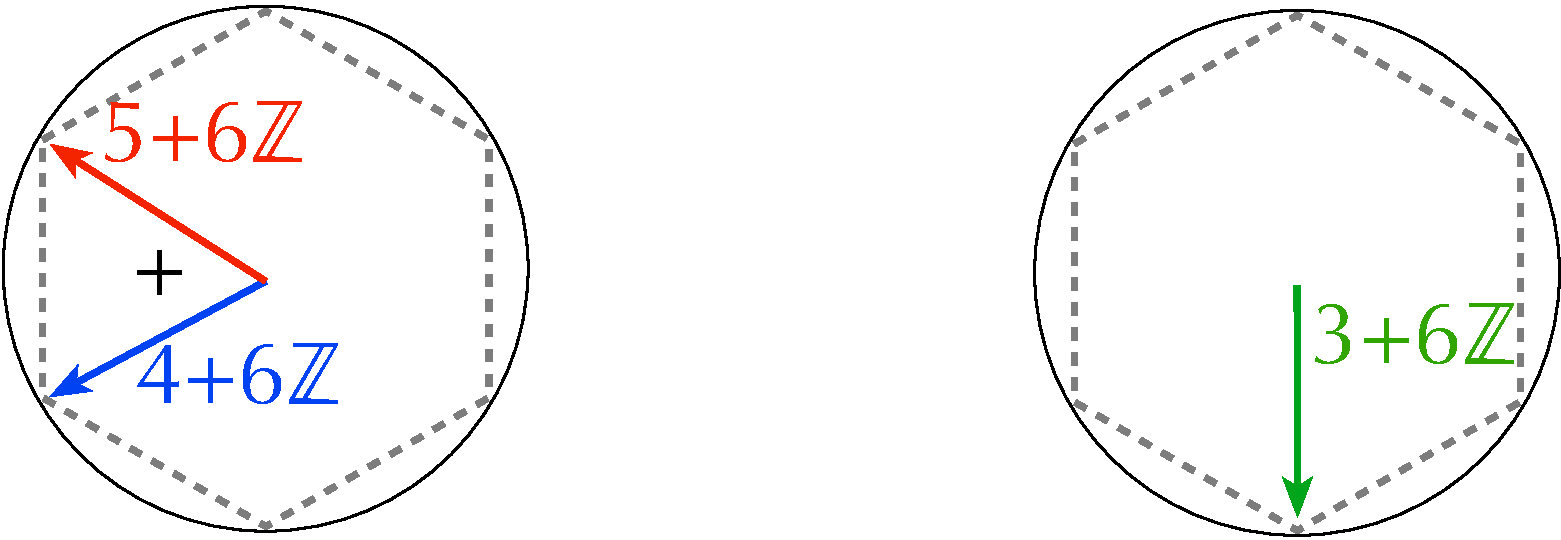
\includegraphics[height=20mm]{pics/cyclicGroup2.pdf}
	\begin{block}{Erinnerung: die zyklische Gruppe}
		\begin{itemize}
		\item Wir erinnern uns an die Gruppe $\ZZ_n$ mit den Elementen
			\begin{align*}
				\cbc{z+n\cdot\ZZ:z\in\ZZ}.
			\end{align*}
		\item Wir haben gesehen, da\ss\ es $n$ verschiedene Elemente gibt:
			\begin{align*}
				0+n\cdot\ZZ,\quad1+n\cdot\ZZ,\quad\cdots,\quad(n-1)+n\cdot\ZZ.
			\end{align*}
		\item Die Addition $+$ ist definiert durch
			\begin{align*}
				(x+n\cdot\ZZ)+(y+n\cdot\ZZ)=(x+y)+n\cdot\ZZ\enspace.
			\end{align*}
		\end{itemize}
	\end{block}
\end{frame}

\begin{frame}\frametitle{Ringe}
	\begin{block}{Der Restklassenring}
		\begin{itemize}
			\item definiere auf $\ZZ_n$ eine Multiplikation durch
				\begin{align*}
					(x+n\cdot\ZZ)\cdot(y+n\cdot\ZZ)=(x\cdot y)+n\cdot\ZZ.
				\end{align*}
			\item Mit dieser Multiplikation ist $\ZZ_n$ ein kommutativer Ring.
			\item Das Einselement ist $1+n\cdot\ZZ$.
		\end{itemize}
	\end{block}
\end{frame}

\begin{frame}\frametitle{Ringe}
	\begin{overprint}
		\onslide<1>	
		\begin{block}{Rechenschema f\ue r die Addition}
			\emph{Aufgabe:} $(x+n\cdot\ZZ)+(y+n\cdot\ZZ)$ ausrechnen.
			\begin{enumerate}
				\item Berechne $z=x+y$.
				\item Dividiere $z$ mit Rest durch $n$:
					\begin{align*}
						z&=q\cdot n+r&&\mbox{mit }0\leq r<n.
					\end{align*}
				\item Das Ergebnis ist $r+n\cdot\ZZ$.
			\end{enumerate}
		\end{block}
		\onslide<2>	
		\begin{block}{Rechenschema f\ue r die Multiplikation}
			\emph{Aufgabe:} $(x+n\cdot\ZZ)\cdot(y+n\cdot\ZZ)$ ausrechnen.
			\begin{enumerate}
				\item Berechne $z=x\cdot y$.
				\item Dividiere $z$ mit Rest durch $n$:
					\begin{align*}
						z&=q\cdot n+r&&\mbox{mit }0\leq r<n.
					\end{align*}
				\item Das Ergebnis ist $r+n\cdot\ZZ$.
			\end{enumerate}
		\end{block}
	\end{overprint}
\end{frame}

\begin{frame}\frametitle{Ringe}
	\hfill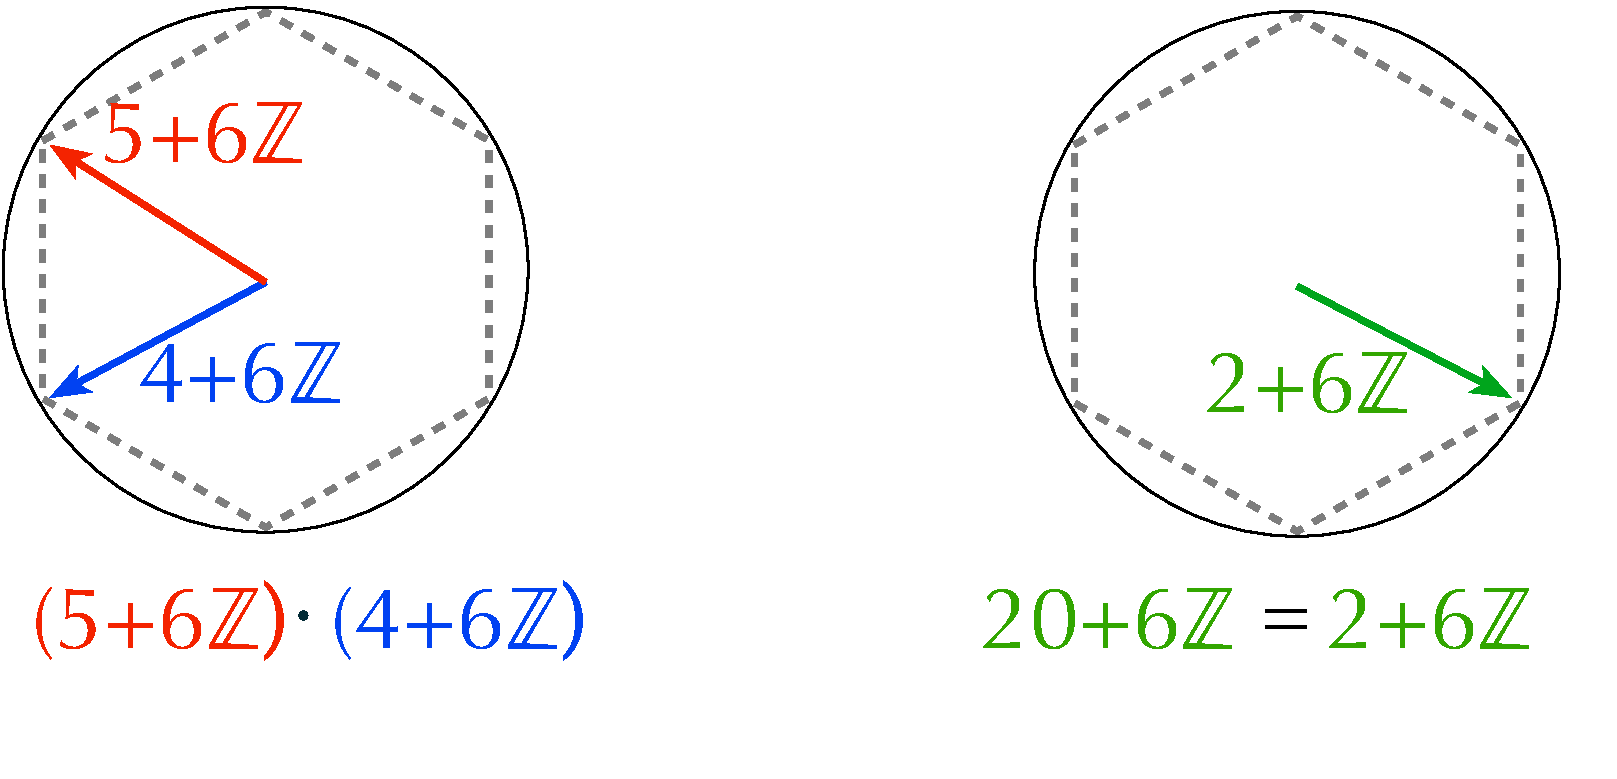
\includegraphics[height=30mm]{pics/cyclicGroup3.pdf}
	\begin{block}{Beispiel}
	\begin{itemize}
		\item Ausrechnen von $(5+6\ZZ)\cdot(4+6\ZZ)$
		\item Wir berechnen $5\cdot 4=20$.
		\item Division mit Rest durch 6:
			\begin{align*}
			20=3\cdot 6+2.
			\end{align*}
		\item \emph{Ergebnis:} $2+6\ZZ$.
	\end{itemize}
	\end{block}
\end{frame}

\begin{frame}\frametitle{Ringe}
	\hfill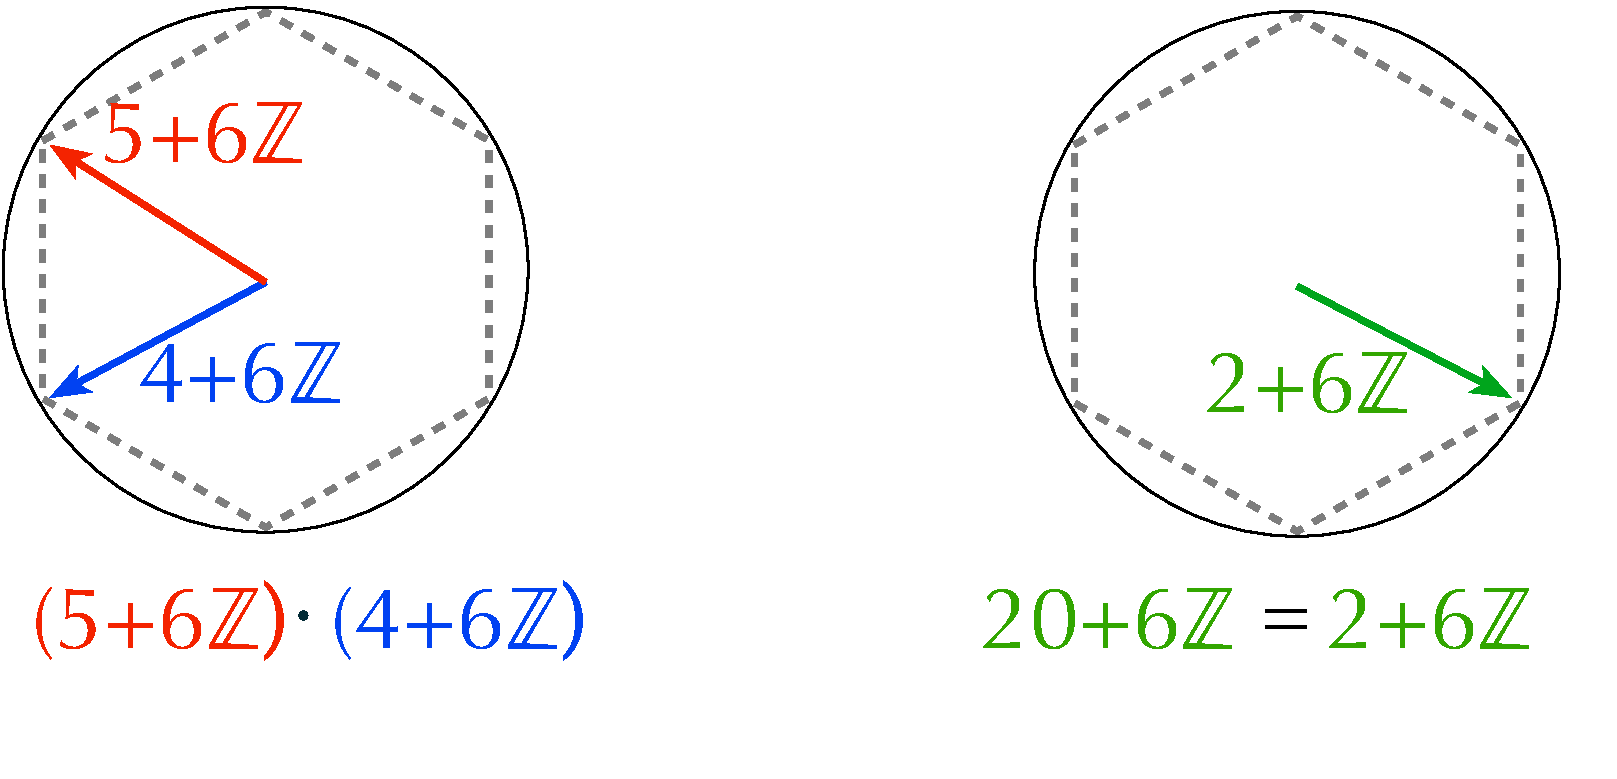
\includegraphics[height=30mm]{pics/cyclicGroup3.pdf}
	\begin{block}{Beispiel}
	\begin{itemize}
		\item Ausrechnen von $(2+6\ZZ)\cdot(3+6\ZZ)$
		\item Wir berechnen $2\cdot 3=6$.
		\item Division mit Rest durch 6:
			\begin{align*}
			6=1\cdot 6+0.
			\end{align*}
		\item \emph{Ergebnis:} $0+6\ZZ$.
	\end{itemize}
	\end{block}
\end{frame}

\begin{frame}\frametitle{Ringe}
\begin{block}{Definition}
	Sei $(R,\oplus,\otimes)$ ein Ring.
	Wir nennen $x\in R$ eine \emph{Einheit}, falls es ein $y\in R$ mit
	\begin{align*}
	y\otimes x=x\otimes y=1
	\end{align*}
gibt.
In diesem Fall hei\ss t $y$ das \emph{Inverse} von $x$.
\end{block}
\end{frame}

\begin{frame}\frametitle{Ringe}
	\begin{block}{Beispiel}
		\begin{itemize}
			\item In dem Ring $(\ZZ,+\,\,\cdot\,)$ sind $1,-1$ Einheiten.
			\item In dem Ring $(\QQ,+,\,\cdot\,)$ sind alle Br\ue che $\frac{x}{y}\in\QQ\setminus\cbc0$ Einheiten und das Inverse zu $\frac{x}{y}$ ist $\frac{y}{x}$.
			\item In dem Ring $(\ZZ_6,+,\,\cdot\,)$ sind nur $1+6\ZZ,5+6\ZZ$ Einheiten.
			\item In jedem Ring ist das Einselement eine Einheit.
			\item Das Nullelement ist niemals eine Einheit.
		\end{itemize}
	\end{block}
\end{frame}

\begin{frame}\frametitle{Ringe}
	\begin{block}{Schreibweisen}
		Sei $(R,\oplus,\otimes)$ ein Ring, $x\in R$ und $\ell\in\NN$.
		Wir schreiben
		\begin{itemize}
			\item $\ell x=\ell\cdot x=\underbrace{x\oplus x\oplus \cdots\oplus x}_{\mbox{$\ell$ mal}}$
			\item $-x$ f\ue r das inverse Element von $x$ bzgl.\ $\oplus$
			\item $-\ell x=-\ell\cdot x=\underbrace{(-x)\oplus (-x)\oplus \cdots\oplus (-x)}_{\mbox{$\ell$ mal}}$
			\item Wenn $x$ eine Einheit ist, schreiben wir $x^{-1}$ f\ue r das Inverse.
			\item $x^\ell=\underbrace{x\otimes x\otimes\cdots\otimes x}_{\mbox{$\ell$ mal}}$
			\item $x^{-\ell}=\underbrace{x^{-1}\otimes x^{-1}\otimes\cdots\otimes x^{-1}}_{\mbox{$\ell$ mal}}$
			\item $R^\times$ ist die Menge aller Einheiten von $R$.
		\end{itemize}
	\end{block}
\end{frame}

\begin{frame}\frametitle{Ringe}
	\begin{block}{Lemma}
		Die Menge $R^\times$ ist zusammen mit der Verkn\ue pfung $\otimes$ eine Gruppe.
	\end{block}
	\begin{block}{Anmerkung}
		\begin{itemize}
			\item Wir nennen $R^\times$ die \emph{Einheitengruppe}.
			\item Es gilt immer $1\in R^\times$.
			\item Wenn $x\in R^\times$, dann auch $x^{-1}\in R^\times$.
		\end{itemize}
	\end{block}
\end{frame}

\begin{frame}\frametitle{Ringe}
	\begin{block}{Beispiel}
		\begin{itemize}
			\item Die Einheitengruppe von $(\ZZ,+,\,\cdot\,)$ ist
				\begin{align*}
					\ZZ^\times=\{1,-1\}
				\end{align*}
			\item Die Einheitengruppe von $(\QQ,+,\,\cdot\,)$ ist
				\begin{align*}
					\QQ^\times=\QQ\setminus\cbc 0
				\end{align*}
		\end{itemize}
	\end{block}
\end{frame}

\begin{frame}\frametitle{Ringe}
	\begin{block}{Proposition}
		Sei $n\geq2$.
		Die Einheitengruppe des Restklassenrings $\ZZ_n$ ist
		\begin{align*}
			\ZZ_n^\times=\cbc{m+n\ZZ:0\leq m<n\mbox{ und }\ggt(m,n)=1}.
		\end{align*}
		Also gilt $|\ZZ_n^\times|=\phi(n)$.
	\end{block}
\end{frame}

\begin{frame}\frametitle{Ringe}
	\begin{block}{Rechenregeln f\ue r Restklassenringe}
		\emph{Aufgabe:} zu $n\geq2$ und $m$ mit $\ggt(m,n)=1$ berechne das Inverse von $m+n\ZZ$ in $\ZZ_n$.
		\begin{itemize}
			\item Bestimme mit dem erweiterten Euklidischen Algorithmus Zahlen $x,y\in\ZZ$ mit
				\begin{align*}
					x\cdot m+y\cdot n=1.
				\end{align*}
			\item Dividiere dann $x$ mit Rest durch $n$:
				\begin{align*}
					x&=q\cdot n+r&&\mbox{mit }0\leq r<n.
				\end{align*}
			\item Das Inverse von $m+n\ZZ$ ist dann
				\begin{align*}
					(m+n\ZZ)^{-1}=r+n\ZZ.
				\end{align*}
		\end{itemize}
	\end{block}
\end{frame}

\begin{frame}\frametitle{Ringe}
	\begin{block}{Beispiel}
		\begin{itemize}
			\item Betrachte $n=12$ und $m=5$.
			\item Erweiterten Euklidischen Algorithmus anwenden:
				\begin{align*}
					12&=2\cdot 5+2&\Rightarrow2&=12-2\cdot 5\\
					5&=2\cdot 2+1&\Rightarrow1&=5-2\cdot 2\\&&&=5-2\cdot(12-2\cdot 5)\\&&&=5\cdot 5-2\cdot 12
				\end{align*}
			\item Also $(5+12\ZZ)^{-1}=5+12\ZZ$.
			\item Die Einheitengruppe ist 
				\begin{align*}
					\ZZ_{12}^\times=\cbc{1+12\ZZ,5+12\ZZ,7+12\ZZ,11+12\ZZ}.
				\end{align*}
		\end{itemize}
	\end{block}
\end{frame}

\begin{frame}\frametitle{Ringe}
	\begin{block}{Beispiel}
		\begin{itemize}
			\item Betrachte $n=14$ und $m=3$.
			\item Erweiterten Euklidischen Algorithmus anwenden:
				\begin{align*}
					14&=4\cdot 3+2&\Rightarrow2&=14-4\cdot 3\\
					3&=1\cdot 2+1&\Rightarrow1&=3-1\cdot 2\\&&&=3-(14-4\cdot 3)\\&&&=5\cdot 3-1\cdot 14
				\end{align*}
			\item Also $(3+14\ZZ)^{-1}=5+14\ZZ$.
			\item Die Einheitengruppe ist 
				\begin{align*}
					\ZZ_{14}^\times=\cbc{1+14\ZZ,3+14\ZZ,5+14\ZZ,9+14\ZZ,11+14\ZZ,13+14\ZZ}.
				\end{align*}
		\end{itemize}
	\end{block}
\end{frame}

\begin{frame}\frametitle{K\oe rper}
	\begin{block}{Definition}
		Ein kommutativer Ring $(R,\oplus,\otimes)$ ist ein \emph{K\oe rper}, falls $R^\times=R\setminus\cbc 0.$
	\end{block}
	\begin{block}{}
		\itshape Ein K\oe rper ist ein kommutativer Ring, in dem jedes Element au\ss er der Null eine Einheit ist.
	\end{block}
\end{frame}

\begin{frame}\frametitle{K\oe rper}
	\begin{block}{Die K\oe rperaxiome}
		Ein K\oe rper ist eine Menge $K$ mit zwei Verkn\ue pfungen
		\begin{align*}
			\oplus:K\times K\to K&&\otimes:K\times K\to K
		\end{align*}
		so da\ss\ 
	\begin{itemize}
		\item $(K,\oplus)$ eine Abelsche Gruppe ist,
		\item $(K\setminus\cbc 0,\otimes)$ eine Abelsche Gruppe ist und
		\item das Distributivgesetz gilt, d.h.\ f\ue r alle $x,y,z\in K$ gilt
			\begin{align*}
				x\otimes(y\oplus z)=x\otimes y\oplus x\otimes z.
			\end{align*}
	\end{itemize}
	\end{block}
\end{frame}

\begin{frame}\frametitle{K\oe rper}
	\begin{block}{Beispiele}
		\begin{itemize}
			\item $(\QQ,+,\,\cdot\,)$ ist ein K\oe rper.
			\item $\ZZ_n$ ist genau dann ein K\oe rper, wenn $n$ eine Primzahl ist.
		\end{itemize}
	\end{block}
\end{frame}

\begin{frame}\frametitle{K\oe rper}
	\begin{block}{Satz}
		Sei $(K,\oplus,\otimes)$ ein endlicher K\oe rper.
		Dann ist $(K^\times,\otimes)$ eine zyklische Gruppe.
	\end{block}
	\begin{block}{Anmerkung}
		\begin{itemize}
			\item In einem endlichen K\oe rper gibt es also ein $q\in K^\times$, so da\ss\
				\begin{align*}
					K^\times&=\cbc{q^\ell:\ell\geq0}.
				\end{align*}
			\item Ein solches Element $q$ nennt man \emph{primitives Element}.
			\item Die Anzahl verschiedener primitiver Elemente ist $\phi(|K|-1)$.
		\end{itemize}
	\end{block}
\end{frame}

\begin{frame}\frametitle{K\oe rper}
	\begin{block}{Beispiel}
		\begin{itemize}
			\item $n=7$ ist eine Primzahl
			\item folglich ist $\ZZ_7$ ein K\oe rper.
			\item die primitiven Elemente sind
				\begin{align*}
					q_1&=3+7\ZZ,&q_2=4+7\ZZ.
				\end{align*}
			\item Beispielsweise rechnen wir die Potenzen von $3+7\ZZ$ aus:
				\begin{align*}
					3^0&=1&3^1&=3&3^2&=9\\
					(3+7\ZZ)^0&=1+7\ZZ& (3+7\ZZ)^1&=3+7\ZZ& (3+7\ZZ)^2&=2+7\ZZ\\\\
					3^3&=27&3^4&=81&3^5&=243\\
				(3+7\ZZ)^3&=6+7\ZZ& (3+7\ZZ)^4&=4+7\ZZ& (3+7\ZZ)^5&=5+7\ZZ \end{align*}
		\end{itemize}
	\end{block}
\end{frame}

\begin{frame}\frametitle{Zusammenfassung}
	\begin{itemize}
		\item Begriff Ring
		\item Restklassenring $\ZZ_n$
		\item Einheitengruppe $R^\times$
		\item K\oe rper
		\item Primitives Element
	\end{itemize}
\end{frame}

\end{document}
